Una vez llevado a cabo el desarrollo teórico de la aplicación y los cálculos necesarios para llegar a los resultados deseados, el siguiente paso será aplicar estos a un emplazamiento concreto, observar los resultados obtenidos y analizarlos para sacar una conclusión.

Éste capítulo también servirá como una guía detallada de uso de la aplicación, explicando la información a introducir en cada paso y como obtenerlos.

La aplicación está disponible a través del enlace \url{http://solarcalc.app} para utilizarse de manera totalmente gratuita.

\section{Obtención de datos del usuario}

El formulario que se le presenta al usuario para que éste introduzca la información de su emplazamiento es el siguiente:
\begin{figure}[ht]
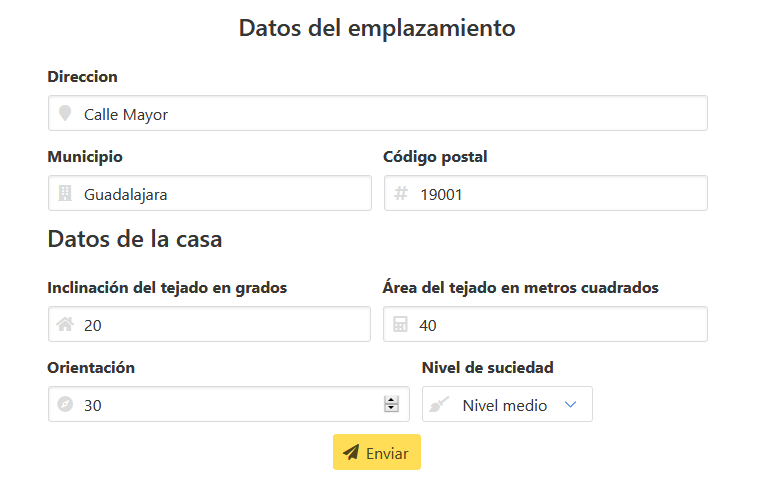
\includegraphics[scale=0.4]{USER_FORM}
\centering
\caption{Formulario web para obtención de datos}
\label{fig:user_form}
\end{figure}

Como se puede observar, el formulario consta de dos partes, por un lado está la dirección como tal, que se utilizará para obtener las coordenadas del emplazamiento y por otro está la configuración física de la superficie destinada a la instalación de los paneles solares.

\subsection{Latitud y longitud a partir de la dirección}

La primera parte del formulario consiste en obtener la información acerca del emplazamiento del usuario, es decir, su latitud y longitud. Estos datos son los que se utilizarán en el código, para obtener la información de la radiación en dicho lugar. El proceso completo para obtener los datos de radiación se describe en \ref{section:adrase_web}

\begin{figure}[ht]

\includegraphics[scale=0.6]{address_form}
\centering
\caption{Campos del formulario para la dirección}
\label{fig:address_form}
\end{figure}

Para ello, el formulario pide una dirección, que no necesariamente tiene que ser la exacta del emplazamiento, sino que se puede utilizar una dirección genérica cercana al lugar donde se va a realizar la instalación, ya que para una distancia relativamente corta la radiación solar no variará de manera notable.

En la sección \ref{section:get_address} se expone en detalle el proceso para obtener las coordenadas en función de la dirección del usuario.

En este caso práctico la dirección que utilizaremos será la de Guadalajara. Para ésta dirección, las coordenadas que Google nos devuelve son:
\begin{itemize}
\item \textbf{Latitud:} $40,632 \degree$.
\item \textbf{Longitud:} $-3.166 \degree$.
\end{itemize}

\subsection{Datos de la superficie destinada a la instalación}

Una vez obtenidas las coordenadas del emplazamiento, es necesario conocer la inclinación, la orientación y el nivel de suciedad de la superficie, para poder realizar el cambio de la radiación en el plano horizontal obtenida anteriormente a la radiación eficiente incidente.

\begin{figure}[ht]
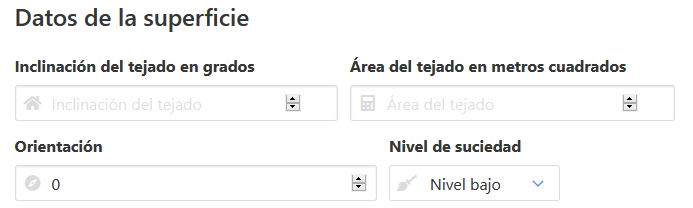
\includegraphics[scale=0.5]{house_form}
\centering
\caption{Campos del formulario para los datos de la superficie}
\label{fig:house_form}
\end{figure}

\newpage

El campo del nivel de suciedad es un desplegable ya que solamente existen 4 niveles, que afectan a los cálculos de una manera específica, como se ha visto en el capítulo teórico, por tanto, debemos limitar la forma en la que el usuario introduce esa información.

\begin{figure}[ht]

\includegraphics[scale=0.6]{dirt_level_select}
\centering
\caption{Campos del formulario para los datos de la superficie}
\label{fig:dirt_level_input}
\end{figure}


Para ello el formulario nos ofrece 4 campos de información:

\begin{itemize}
\item \textbf{Inclinación en grados:} Para obtener la inclinación de la superficie en grados se puede utilizar cualquier smartphone actual dotado con un sensor giroscópico y una aplicación de tipo nivel, algún dispositivo de medición de ángulos como un transportador.
\item \textbf{Orientación:} Para la obtener la orientación de la superficie se puede utilizar una brújula, ya sea analógica o digital. Se considera que 0 grados es el SUR.
\item \textbf{Área del tejado:} Una estimación aproximada del área disponible el área que se desea cubrir con paneles solares.
\item \textbf{Nivel de suciedad:} Este campo es el mas subjetivo y será a criterio del usuario. Se recomienda realizar cálculos con el peor caso para establecer un margen pero, no obstante, si se conoce con seguridad cuál es el nivel de suciedad de la zona, se ha de usar éste.
\end{itemize}

Un proceso detallado de como obtener los valores de inclinación y orientación se describe a continuación

\subsection{Obtención de la inclinación y orientación de la superficie}

\subsubsection{Medición de la inclinación}

En la aplicación se presentan dos campos dentro del formulario que debe rellenar el usuario, que requieren introducir la inclinación y la orientación de la superficie donde se va a instalar el generador fotovoltaico.

Para ello, existen multitud de aplicaciones gratuitas en la tienda de aplicaciones tanto de Android como de iOS. En este caso, se va a mostrar un ejemplo con un dispositivo Android, pero esto se puede trasladar igualmente a un dispositivo iOS.

La aplicación que se va a utilizar se llama \textit{Angle Meter}, y la empresa que lo desarrolla se llama \textit{Smart Tool Factory}. Se encuentra en la Play Store de Android de manera gratuita.

Cuando se abre la aplicación por primera vez, encontramos lo siguiente:

\begin{figure}[H]
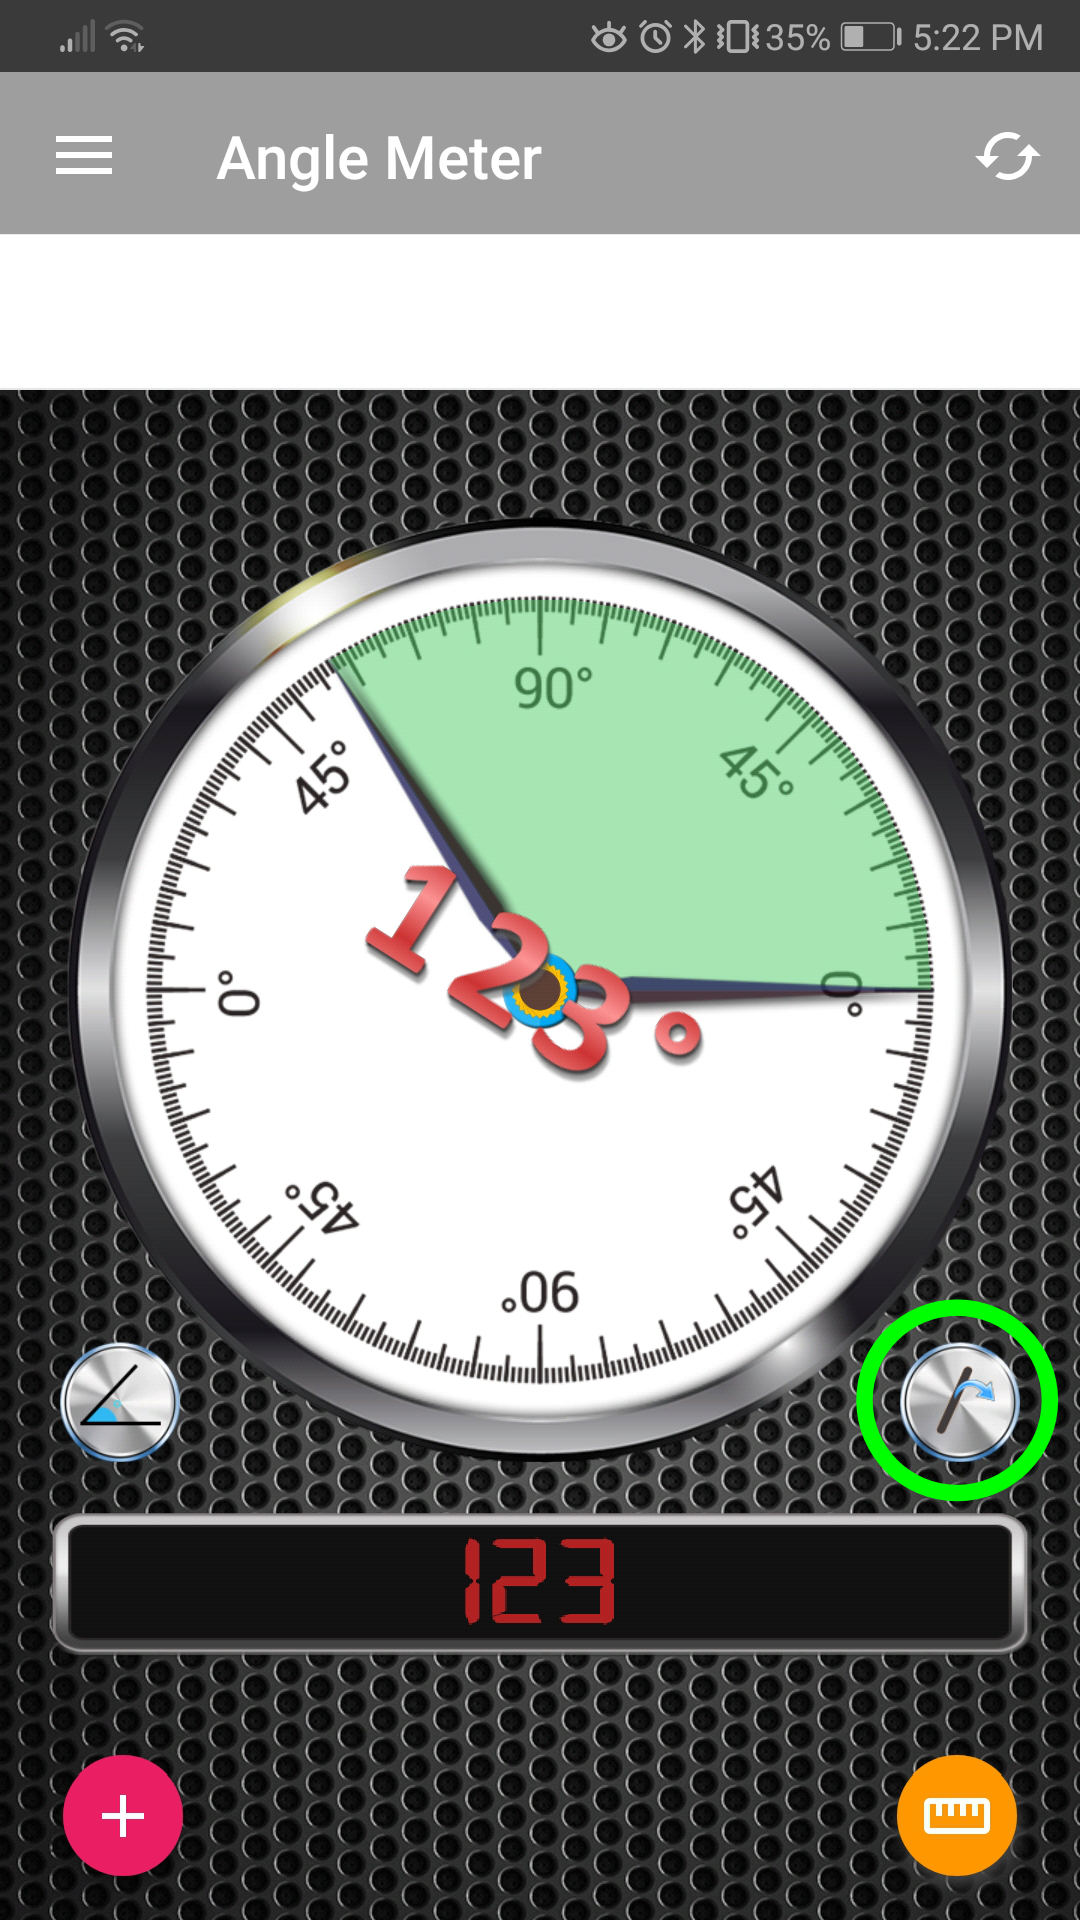
\includegraphics[scale=0.2]{app_homescreen}
\centering
\caption{Pantalla de inicio de la aplicación}
\end{figure}

A continuación, pulsamos el botón que sale remarcado con un círculo verde, lo que hará que cambie el modo de medición de ángulos a inclinación, que es el necesario para obtener el dato de la inclinación. Cuando la aplicación cambie a ese modo, se verá de la siguiente manera:

\begin{figure}[H]
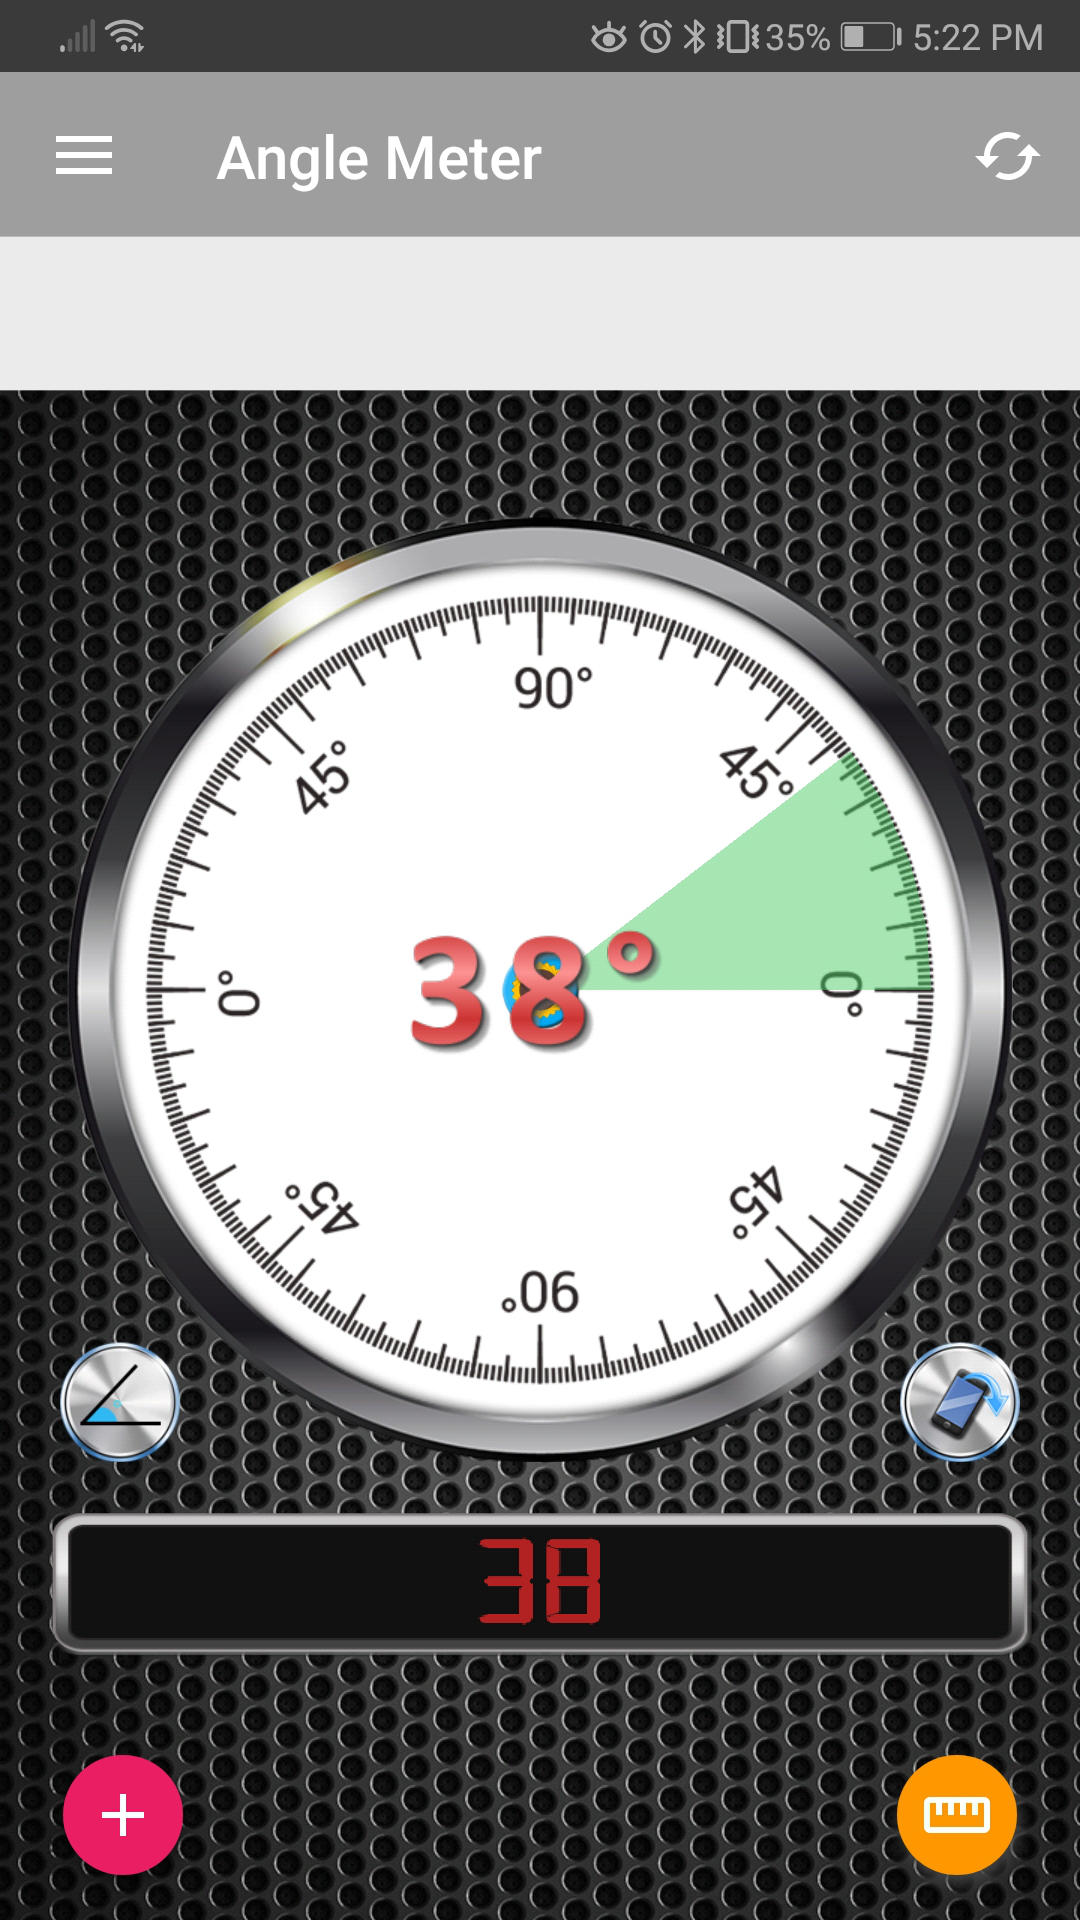
\includegraphics[scale=0.2]{app_angle}
\centering
\caption{Medición de ángulo}
\end{figure}

A continuación, el dispositivo se debe colocar según la figura que se muestra abajo, teniendo en cuenta que la imagen se muestra con una perspectiva perpendicular a la superficie.
\begin{figure}[H]
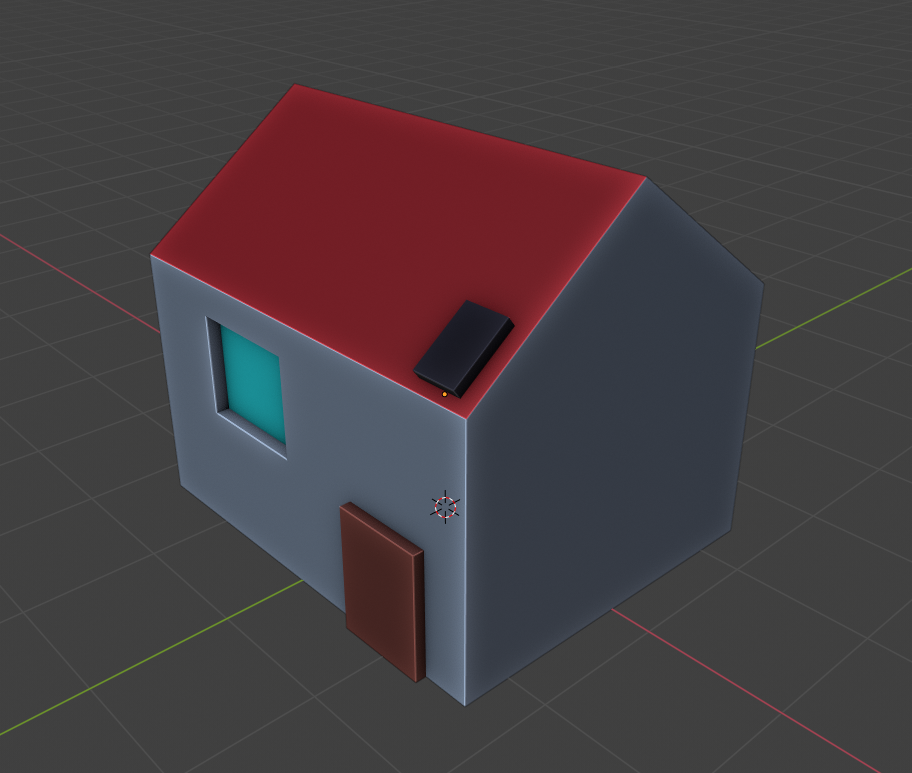
\includegraphics[scale=0.4]{phone_placement}
\centering
\caption{Posición del dispositivo}
\end{figure}

De esta manera, obtenemos la inclinación de la superficie en grados.

\subsubsection{Medición de la orientación}

Para obtener la orientación de la superficie, debemos cambiar una vez más el modo de funcionamiento de la aplicación, dejando el dispositivo en la mismo posición que en la medición de inclinación.

Para ello, abrimos el menú desde la izquierda y pulsamos en la opción llamada \textit{Compass}, como se muestra en la siguiente figura.

\begin{figure}[H]
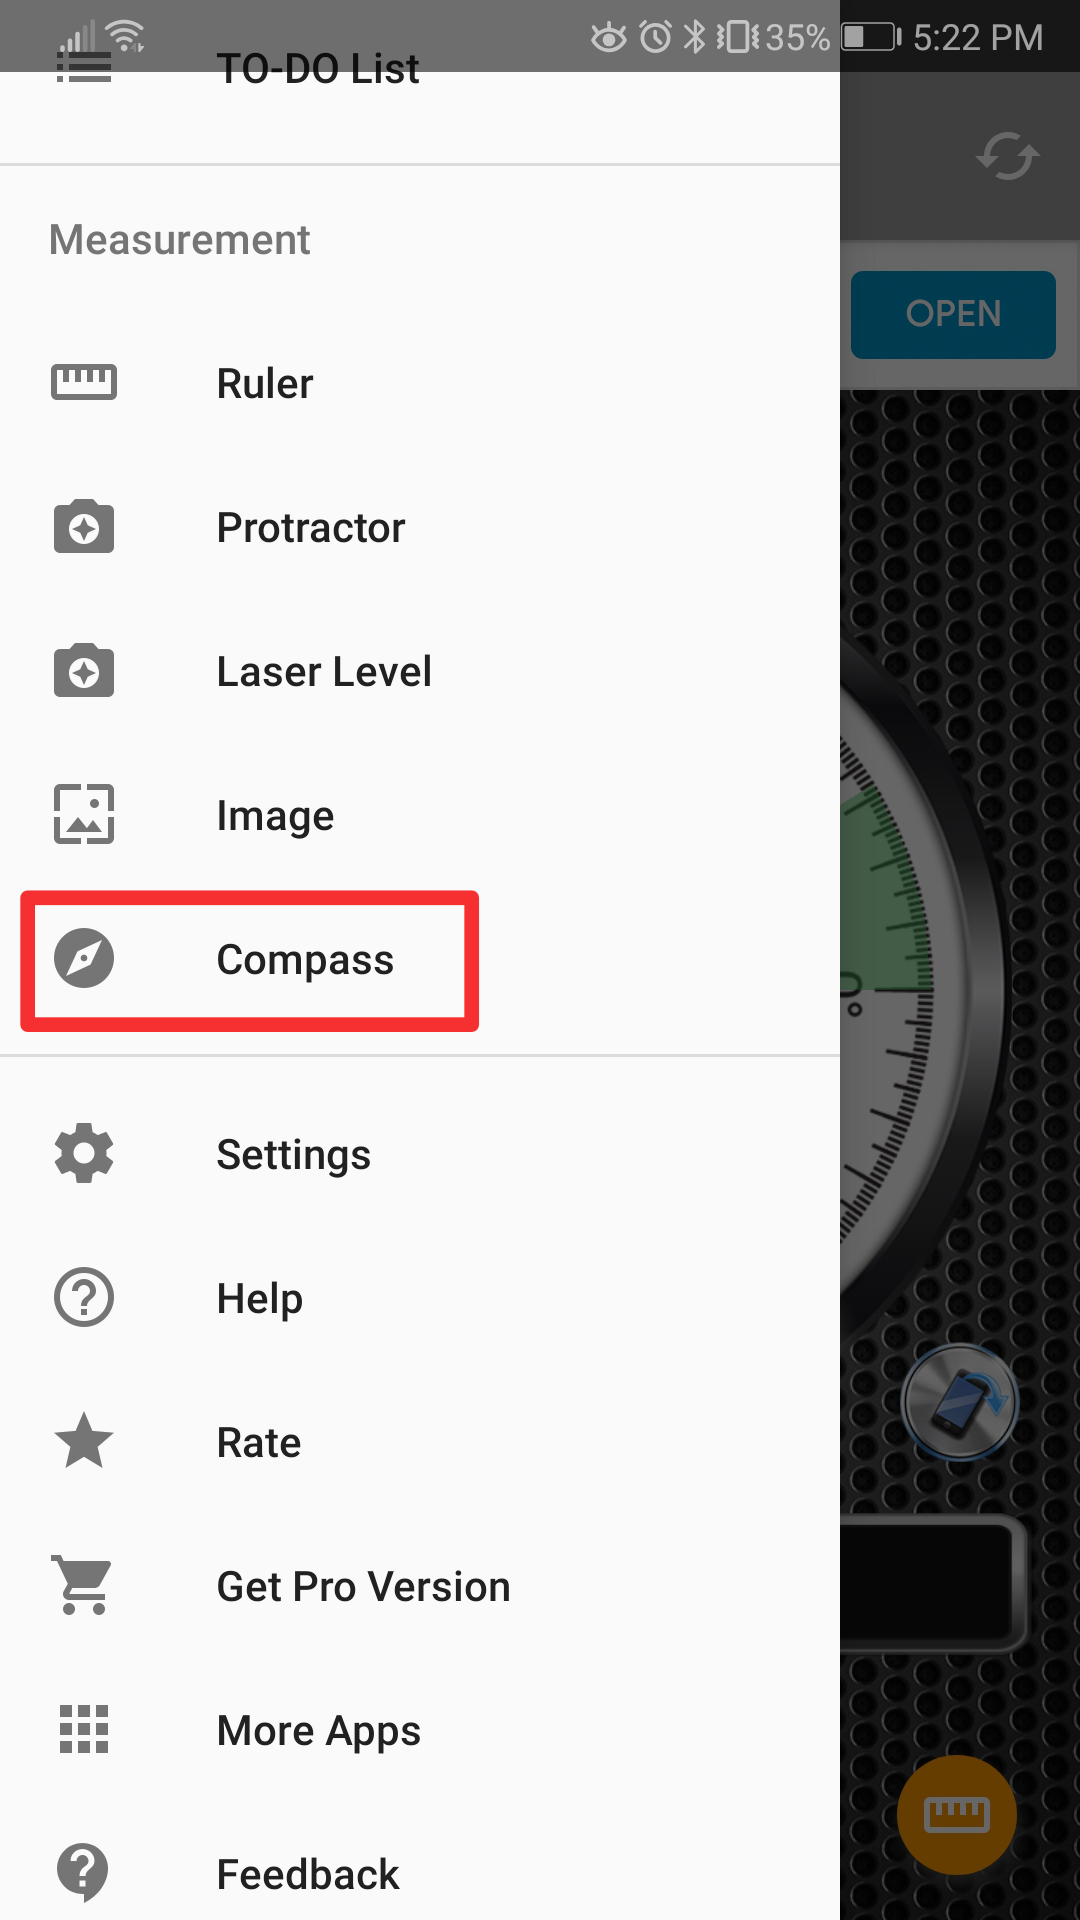
\includegraphics[scale=0.2]{app_menu_compass}
\centering
\caption{Opción brújula del menú}
\end{figure}

Una vez abierta la brújula, observamos la medición que nos muestra en la parte inferior central de la pantalla. A esa medición debemos restarle 180 $\degree$ para obtener el valor que necesita la aplicación de cálculo. Es decir, si observamos una orientación de 193 $\degree$, en el formulario introduciremos 13 $\degree$. En la figura de abajo se muestra como se ve la pantalla de la brújula.

\begin{figure}[H]
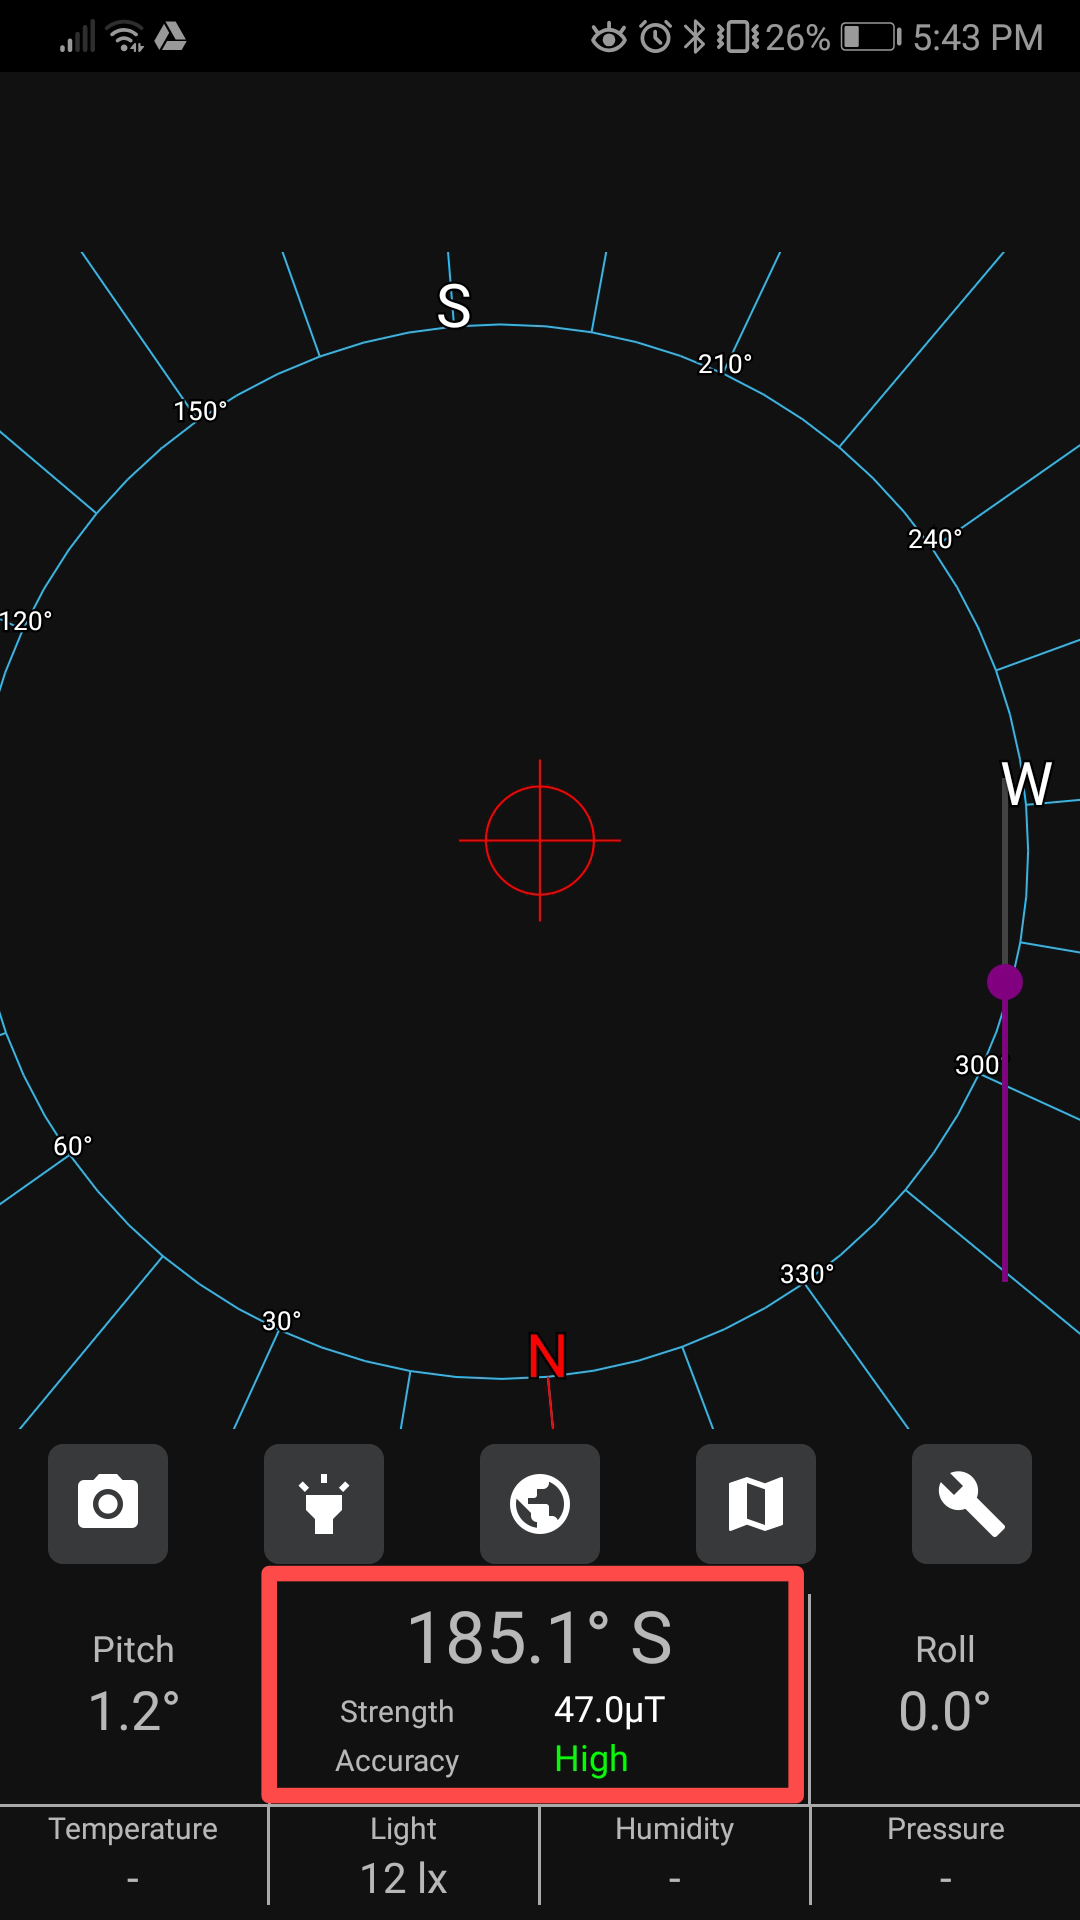
\includegraphics[scale=0.2]{app_compass}
\centering
\caption{Opción brújula del menú}
\end{figure}

\section {Aplicación de los datos al proceso de cálculo}

En la sección anterior hemos recogido los datos que un usuario ha introducido a través del formulario. Estos datos son:
\begin{itemize}
\item \textbf{Latitud:} $40,632 \degree$.
\item \textbf{Longitud:} $-3.166 \degree$.
\item \textbf{Inclinación de la superficie:} $20 \degree$.
\item \textbf{Área de la superficie:} $40 m^2 $.
\item \textbf{Orientación de la superficie:} $30 \degree$ SUR.
\item \textbf{Nivel de suciedad:} Medio.
\end{itemize}

A continuación, utilizaremos estos datos para recorrer numéricamente el proceso teórico descrito en el capítulo anterior. 

\subsection{Valores medios mensuales de radiación global}

Tal y como se menciona en la sección \ref{section:get_global_rad}, el primer paso para poder llevar a cabo el proceso de cálculo de la radiación incidente efectiva es obtener la radiación global media para cada uno de los doce meses, en el emplazamiento indicado por el usuario.

Para las coordenadas introducidas por el usuario, el punto con información mas cercano que tenemos es de latitud  $40,57 \degree$ y longitud $-3.16 \degree$. 

El proceso de obtención de los siguientes valores se describe en detalle en la sección \ref{section:adrase_web}.

Para este punto, los valores de irradiación media son:
\begin{table}[ht]
\centering
\begin{tabular}{|l|l|l|l|l|l|l|l|l|l|l|l|l|}
\hline
$kWh/m^2$   & Ene & Feb & Mar & Abr & May & Jun & Jul & Ago & Sept & Oct & Nov & Dic \\ \hline
Valor medio & 2,0 & 3,1 & 4,8 & 5,7 & 6,8 & 8,0 & 7,8 & 6,8 & 5,1  & 3,5 & 2,2 & 1,7 \\ \hline
\end{tabular}
\label{tab:mean_values_monthly}
\caption{Irradiación global media mensual}
\end{table}

\begin{figure}[ht]
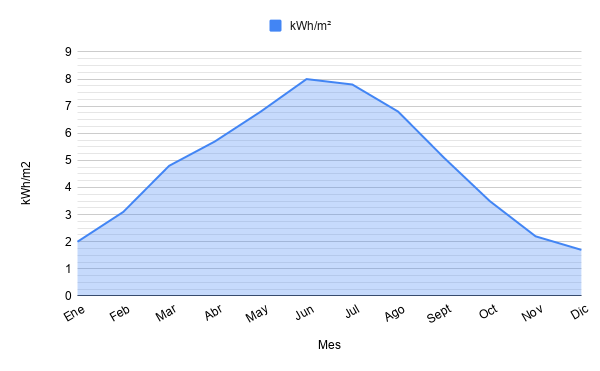
\includegraphics[scale=0.5]{global_monthly_rad}
\centering
\caption{Radiación global en el emplazamiento}
\label{fig:mean_values_monthly}
\end{figure}

\subsection{Irradiancia extra-terrestre diaria}

Además, por otro lado, para poder continuar con el proceso de cálculo, es necesario calcular la irradiancia extra-terrestre diaria, utilizando la latitud indicada por el usuario y los días promedio de la tabla \ref{tab:dias_promedio}.
En las ecuaciones de la sección \ref{section:extra-irrad} se indican los pasos a seguir y el resultado es:
\begin{table}[ht]
\centering
\begin{tabular}{|l|l|l|l|l|l|l|l|l|l|l|l|l|}
\hline
$kW/m^2$   & Ene & Feb & Mar & Abr & May & Jun & Jul & Ago & Sept & Oct & Nov & Dic \\ \hline
$B_{0d}(0)$ & 4,12 & 5,48 & 7,47 & 9,57 & 11,01 & 11,59 & 11,26 & 10,01 & 8,05 & 5,90  & 4,30 & 3,58 \\ \hline
\end{tabular}
\label{tab:extra_irrad_values}
\caption{Irradiancia extra-terrestre diaria}
\end{table}

\begin{figure}[ht]
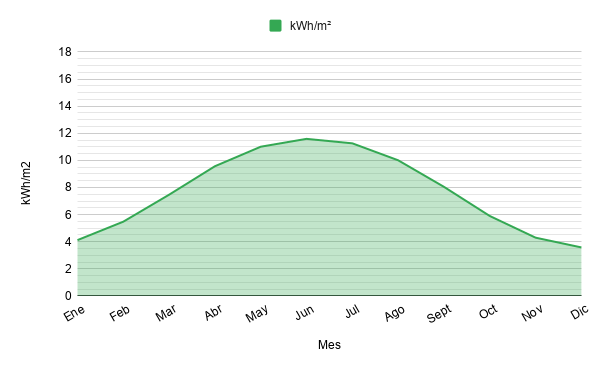
\includegraphics[scale=0.5]{extra_terrestrial_rad}
\centering
\caption{Irradiación extra-terrestre}
\label{fig:mean_values_monthly}
\end{figure}

\subsection{Separación de la radiación global horizontal en sus componentes}

Una vez conocidos los valores mensuales de la radiación global en el plano horizontal, el siguiente paso se centra en separar la radiación global en sus dos componentes, la directa y la difusa, tal y como se explica en la sección \ref{section:radiation_components}.

Como podemos observar en la ecuación \ref{eqn:ktd}, el primer paso para separar la irradiación global en sus dos componentes es calcular el índice de claridad, para que posteriormente calculemos la fracción de radiación difusa. 

Si aplicamos dicha ecuación a los resultados anteriores obtenemos los siguiente resultados:

\begin{table}[ht]
\centering
\begin{tabular}{|l|l|l|l|l|l|l|l|l|l|l|l|l|}
\hline
    & Ene & Feb & Mar & Abr & May & Jun & Jul & Ago & Sept & Oct & Nov & Dic \\ \hline
$K_{Td}$ & 0,485 & 0,565 & 0,642 & 0,595 & 0,617 & 0,690 & 0,692 & 0,679 & 0,632 & 0,592 & 0,511  & 0,461  \\ \hline
\end{tabular}
\label{tab:clarity_index}
\caption{Índice de claridad}
\end{table}

\begin{figure}[ht]
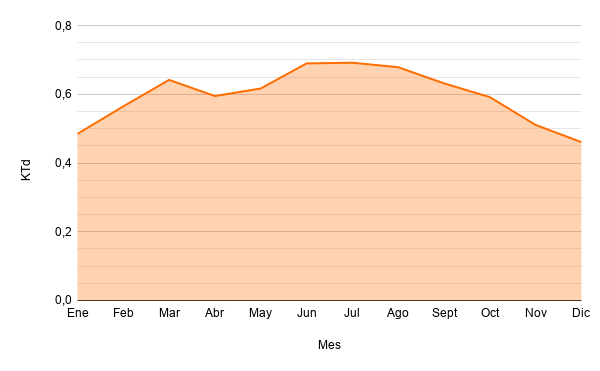
\includegraphics[scale=0.5]{ktd}
\centering
\caption{Índice de claridad}
\label{fig:clarity_index}
\end{figure}


A continuación, utilizando la ecuación de Page \ref{eqn:page}, con el índice de claridad calculado, podemos calcular la fracción de difusa:

\begin{table}[ht]
\centering
\begin{tabular}{|l|l|l|l|l|l|l|l|l|l|l|l|l|}
\hline
   		& Ene   & Feb   & Mar   & Abr   & May   & Jun   & Jul   & Ago   & Sept  & Oct   & Nov    & Dic    \\ \hline
$F_{D}$ & 0,452 & 0,361 & 0,274 & 0,327 & 0,302 & 0,220 & 0,218 & 0,232 & 0,285 & 0,330 & 0,421  & 0,478  \\ \hline
\end{tabular}
\label{tab:difuse_part}
\caption{Fracción de difusa}
\end{table}

\begin{figure}[H]
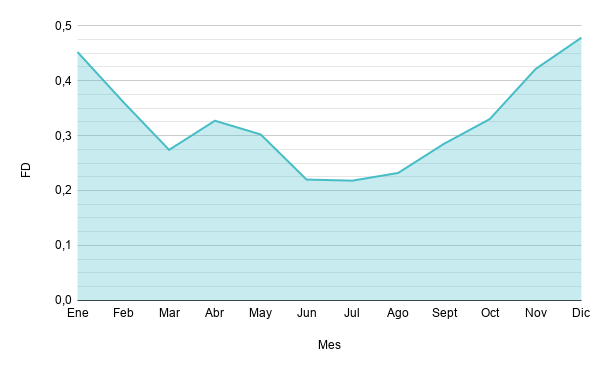
\includegraphics[scale=0.5]{diffuse_fraction}
\centering
\caption{Fracción de difusa}
\label{fig:difuse_part}
\end{figure}

Como era de esperar, se observa que la fracción de difusa es más elevada en los meses con mayor nubosidad y menos intensidad solar.

\subsubsection{Cálculo de las componentes de la radiación  en el plano horizontal}

Con estos valores, utilizando las ecuaciones \ref{eqn:rad_difusa} y \ref{eqn:rad_directa} podemos obtener las dos componentes de la radiación en el plano horizontal.

\begin{table}[ht]
\centering
\begin{tabular}{|l|l|l|l|l|l|l|l|l|l|l|l|l|}
\hline
$kWh/m^2$  & Ene   & Feb   & Mar   & Abr   & May   & Jun   & Jul   & Ago   & Sept  & Oct   & Nov    & Dic    \\ \hline
$B_{d}(0)$ & 1,096 & 1,980 & 3,484 & 3,835 & 4,745 & 6,239 & 6,103 & 5,220 & 3,647 & 2,344 & 1,272  & 0,886  \\ \hline
$D_{d}(0)$ & 0,904 & 1,120 & 1,316 & 1,865 & 2,055 & 1,761 & 1,697 & 1,580 & 1,453 & 1,156 & 0,928  & 0,814  \\ \hline
\end{tabular}
\label{tab:rad_components}
\caption{Irradiación directa y difusa en el plano horizontal}
\end{table}

\begin{figure}[H]
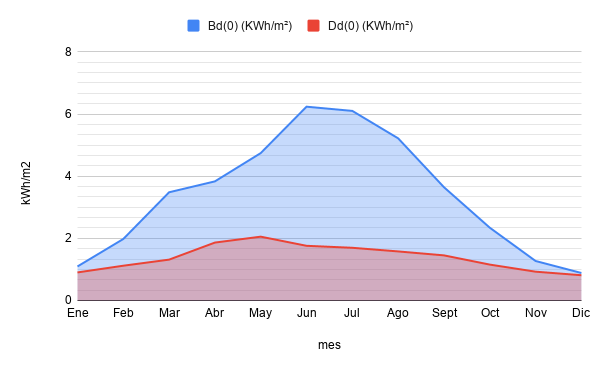
\includegraphics[scale=0.5]{horizontal_rad_comps_abs}
\centering
\caption{Componentes de la irradiación en el plano horizontal}
\label{fig:rad_components_abs}
\end{figure}

\begin{figure}[H]
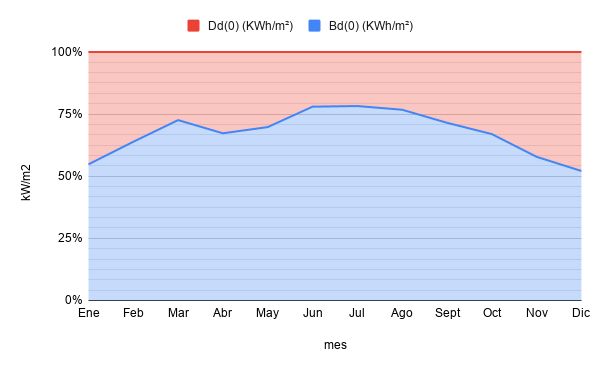
\includegraphics[scale=0.5]{horizontal_rad_comps_percent}
\centering
\caption{Componentes de la irradiación en el plano horizontal}
\label{fig:rad_components_percent}
\end{figure}

La primera gráfica muestra los valores absolutos de las dos componentes, que la segunda muestra el porcentaje de cada una de las dos componentes. Una vez más, se observa una aportación mayor de la radiación difusa en los meses de invierno.

\subsection{Irradiancia en la superficie inclinada}

El término irradiancia ($W/m^2$) se refiere a la magnitud utilizada para describir la potencia incidente por unidad de superficie de cualquier tipo de radiación, en este caso la solar. En cambio, el término irradiación ($Wh/m^2$) es una energía por unidad de área. 

Sin embargo, como la evolución de la radiación solar a lo largo de una hora es relativamente lenta, podemos asumir que la irradiación solar durante esa hora coincide con el valor media de la irradiancia de dicha hora y utilizar los dos términos de manera equivalente.

\subsubsection{Irradiancia en el plano horizontal}
Conociendo ya los valores diarios de la radiación directa y difusa en el plano horizontal, el próximo paso es obtener los valores horarios de irradiancia, tanto directa como difusa, en el plano horizontal para poder llevar a cabo posteriormente, la traslación de estos valores al plano inclinado.El proceso se describe detalladamente en las secciones \ref{section:3.5.1} y \ref{section:3.5.2}.

Al tratarse de 24 valores horarios, para cada uno de los 12 meses, en total tendríamos 288 valores. Por tanto, y con el fin de no saturar este documento con demasiado valores, se van a indicar los resultados de solamente uno de los meses, en concreto de julio. Estos resultados se muestran en la tabla \ref{tab:hourly_horizontal_values}

\begin{figure}[H]
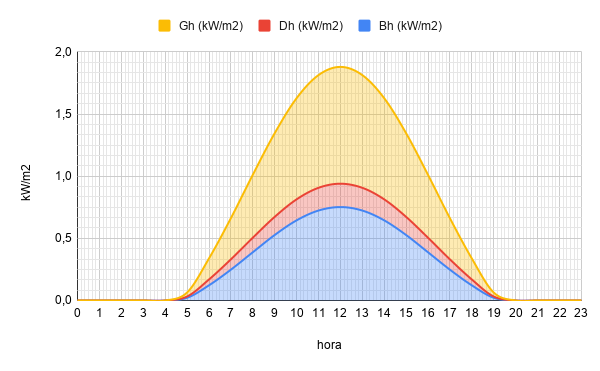
\includegraphics[scale=0.7]{july_hourly_horizontal}
\centering
\caption{Irradiancia para el día promedio del mes de julio}
\label{fig:hourly_horizontal_values}
\end{figure}

\begin{table}[H]
\centering
\begin{tabular}{|c|r|r|r|r|r|}
\hline
 hora
 &
  \multicolumn{1}{c|}{$r_D$} &
  \multicolumn{1}{c|}{$r_G$} &
  \multicolumn{1}{c|}{\begin{tabular}[c]{@{}c@{}}$B(0)$\\ ($kW/m^2$)\end{tabular}} &
  \multicolumn{1}{c|}{\begin{tabular}[c]{@{}c@{}}$D(0)$\\ ($kW/m^2$)\end{tabular}} &
  \multicolumn{1}{c|}{\begin{tabular}[c]{@{}c@{}}$G(0)$\\ ($kW/m^2$)\end{tabular}} \\ \hline
0 & -0,056 & -0,027 & 0     & 0     & 0     \\ \hline
1 & -0,053 & -0,026 & 0     & 0     & 0     \\ \hline
2 & -0,045 & -0,024 & 0     & 0     & 0     \\ \hline
3 & -0,031 & -0,018 & 0     & 0     & 0     \\ \hline
4 & -0,014 & -0,009 & 0     & 0     & 0     \\ \hline
5 & 0,006  & 0,004  & 0,022 & 0,010 & 0,032 \\ \hline
6 & 0,027  & 0,022  & 0,122 & 0,047 & 0,169 \\ \hline
7 & 0,049  & 0,042  & 0,248 & 0,083 & 0,331 \\ \hline
8 & 0,069  & 0,065  & 0,388 & 0,117 & 0,506 \\ \hline
9 & 0,086  & 0,086  & 0,527 & 0,146 & 0,673 \\ \hline
10 & 0,099  & 0,104  & 0,645 & 0,169 & 0,814 \\ \hline
11 & 0,108  & 0,116  & 0,724 & 0,183 & 0,907 \\ \hline
12 & 0,111  & 0,121  & 0,752 & 0,188 & 0,940 \\ \hline
13 & 0,108  & 0,116  & 0,724 & 0,183 & 0,907 \\ \hline
14 & 0,099  & 0,104  & 0,645 & 0,169 & 0,814 \\ \hline
15 & 0,086  & 0,086  & 0,527 & 0,146 & 0,673 \\ \hline
16 & 0,069  & 0,065  & 0,388 & 0,117 & 0,506 \\ \hline
17 & 0,049  & 0,042  & 0,248 & 0,083 & 0,331 \\ \hline
18 & 0,027  & 0,022  & 0,122 & 0,047 & 0,169 \\ \hline
19 & 0,006  & 0,004  & 0,022 & 0,010 & 0,032 \\ \hline
20 & -0,014 & -0,009 & 0     & 0     & 0     \\ \hline
21 & -0,031 & -0,018 & 0     & 0     & 0     \\ \hline
23 & -0,045 & -0,024 & 0     & 0     & 0     \\ \hline
23 & -0,053 & -0,026 & 0     & 0     & 0     \\ \hline
\end{tabular}
\caption{Irradiancia directa, difusa y global en el plano horizontal para el día promedio del mes de julio \label{tab:hourly_horizontal_values}}
\end{table}

\subsubsection{Traslación de los valores al plano inclinado}

Una vez obtenidos los valores horarios en el plano horizontal, podemos trasladar estos al plano inclinado con el proceso descrito de la ecuación \ref{eqn:B_beta_alpha} hasta la ecuación \ref{eqn:ang_incid}.

\begin{table}[H]
\centering
\begin{tabular}{|c|r|r|r|r|r|}
\hline
hora
 &
   \multicolumn{1}{c|}{\begin{tabular}[c]{@{}c@{}}$B(\beta, \alpha)$\\ ($kW/m^2$)\end{tabular}} &
  \multicolumn{1}{c|}{\begin{tabular}[c]{@{}c@{}}$D^C(\beta, \alpha)$\\ ($kW/m^2$)\end{tabular}} &
  \multicolumn{1}{c|}{\begin{tabular}[c]{@{}c@{}}$D^I(\beta, \alpha)$\\ ($kW/m^2$)\end{tabular}} &
  \multicolumn{1}{c|}{\begin{tabular}[c]{@{}c@{}}$D(\beta, \alpha)$\\ ($kW/m^2$)\end{tabular}} &
  \multicolumn{1}{c|}{\begin{tabular}[c]{@{}c@{}}$G(\beta, \alpha)$\\ ($kW/m^2$)\end{tabular}}  \\ \hline
0  & 0     & 0     & 0     & 0     & 0     \\ \hline
1  & 0     & 0     & 0     & 0     & 0     \\ \hline
2  & 0     & 0     & 0     & 0     & 0     \\ \hline
3  & 0     & 0     & 0     & 0     & 0     \\ \hline
4  & 0     & 0     & 0     & 0     & 0     \\ \hline
5  & 0     & 0     & 0,006 & 0,006 & 0,006 \\ \hline
6  & 0     & 0     & 0,027 & 0,027 & 0,027 \\ \hline
7  & 0,12  & 0,018 & 0,044 & 0,062 & 0,184 \\ \hline
8  & 0,280 & 0,042 & 0,057 & 0,099 & 0,379 \\ \hline
9  & 0,448 & 0,067 & 0,065 & 0,132 & 0,580 \\ \hline
10 & 0,603 & 0,091 & 0,069 & 0,160 & 0,763 \\ \hline
11 & 0,721 & 0,108 & 0,072 & 0,180 & 0,901 \\ \hline
12 & 0,786 & 0,118 & 0,072 & 0,190 & 0,977 \\ \hline
13 & 0,787 & 0,119 & 0,072 & 0,191 & 0,978 \\ \hline
14 & 0,724 & 0,109 & 0,070 & 0,179 & 0,903 \\ \hline
15 & 0,610 & 0,092 & 0,065 & 0,156 & 0,767 \\ \hline
16 & 0,463 & 0,069 & 0,057 & 0,127 & 0,589 \\ \hline
17 & 0,304 & 0,046 & 0,044 & 0,090 & 0,394 \\ \hline
18 & 0,156 & 0,023 & 0,027 & 0,050 & 0,206 \\ \hline
19 & 0,033 & 0,005 & 0,006 & 0,011 & 0,044 \\ \hline
20 & 0     & 0     & 0     & 0     & 0     \\ \hline
21 & 0     & 0     & 0     & 0     & 0     \\ \hline
22 & 0     & 0     & 0     & 0     & 0     \\ \hline
23 & 0     & 0     & 0     & 0     & 0     \\ \hline
\end{tabular}
\caption{Irradiancia directa, difusa y global en el plano inclinado, para el día promedio del mes de julio \label{tab:hourly_tilted_values}}
\end{table}

\begin{figure}[H]
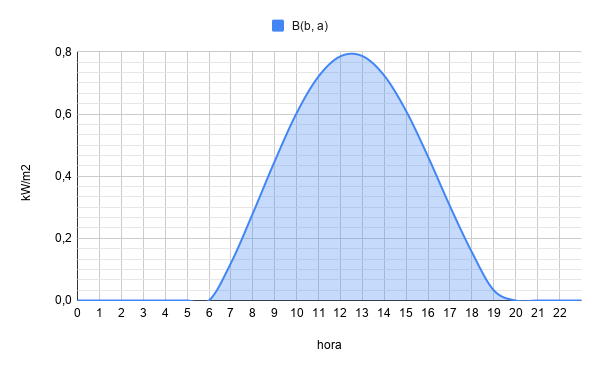
\includegraphics[scale=0.5]{bnoef}
\centering
\caption{Irradiancia directa  en el plano inclinado}
\label{fig:hourly_bef}
\end{figure}

\begin{figure}[H]
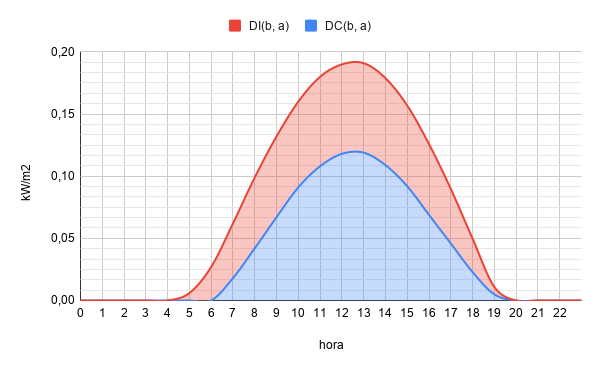
\includegraphics[scale=0.5]{dcnoef_dinoef}
\centering
\caption{Componentes de la irradiancia difusa en el plano inclinado}
\label{fig:hourly_bef}
\end{figure}

\begin{figure}[H]
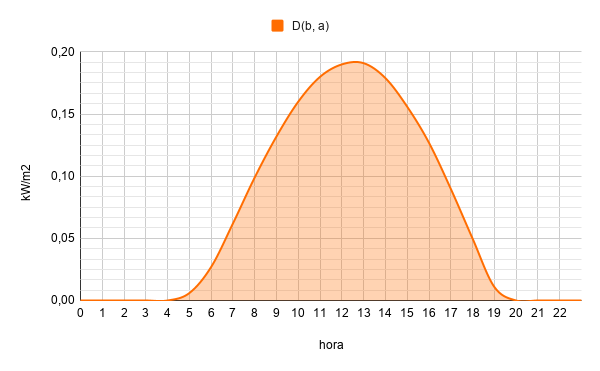
\includegraphics[scale=0.5]{dnoef}
\centering
\caption{Irradiancia difusa en el plano inclinado}
\label{fig:hourly_bef}
\end{figure}

\begin{figure}[H]
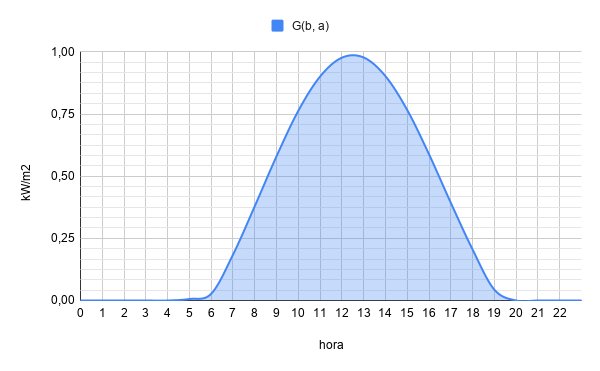
\includegraphics[scale=0.5]{gnoef}
\centering
\caption{Irradiancia global en el plano inclinado}
\label{fig:hourly_bef}
\end{figure}


Como se  puede observar, a diferencia de la irradiancia en el plano horizontal, estos resultados no son simétricos respecto al mediodía ya que ahora está afectando la orientación de la superficie, que no está orientada totalmente hacia el sur.

\subsection{Pérdidas por ángulo de incidencia y suciedad}

Habiendo calculado los valores de irradiancia horaria en la superficie inclinada, el siguiente paso consiste en aplicar las pérdidas por ángulo de incidencia y suciedad, mediante el proceso descrito en la sección \ref{section:3.5.3}. Los resultados del proceso se muestran en la tabla \ref{tab:hourly_tilted_ef_values}.

\begin{table}[H]
\centering
\begin{tabular}{|c|r|r|r|r|r|}
\hline
  hora &
   \multicolumn{1}{c|}{\begin{tabular}[c]{@{}c@{}}$B_{ef}(\beta, \alpha)$\\ ($kW/m^2$)\end{tabular}} &
  \multicolumn{1}{c|}{\begin{tabular}[c]{@{}c@{}}$D^C_{ef}(\beta, \alpha)$\\ ($kW/m^2$)\end{tabular}} &
  \multicolumn{1}{c|}{\begin{tabular}[c]{@{}c@{}}$D^I_{ef}(\beta, \alpha)$\\ ($kW/m^2$)\end{tabular}} &
  \multicolumn{1}{c|}{\begin{tabular}[c]{@{}c@{}}$D_{ef}(\beta, \alpha)$\\ ($kW/m^2$)\end{tabular}} &
  \multicolumn{1}{c|}{\begin{tabular}[c]{@{}c@{}}$G_{ef}(\beta, \alpha)$\\ ($kW/m^2$)\end{tabular}}  \\ \hline
0  & 0     & 0     & 0     & 0     & 0        \\ \hline
1  & 0     & 0     & 0     & 0     & 0        \\ \hline
2  & 0     & 0     & 0     & 0     & 0        \\ \hline
3  & 0     & 0     & 0     & 0     & 0        \\ \hline
4  & 0     & 0     & 0     & 0     & 0        \\ \hline
5  & 0     & 0     & 0,006 & 0,006 & 0,006    \\ \hline
6  & 0     & 0     & 0,025 & 0,025 & 0,025    \\ \hline
7  & 0,076 & 0,011 & 0,041 & 0,052 & 0,128    \\ \hline
8  & 0,243 & 0,037 & 0,052 & 0,089 & 0,3314   \\ \hline
9 & 0,422 & 0,064 & 0,059 & 0,123 & 0,545    \\ \hline
10 & 0,583 & 0,088 & 0,064 & 0,152 & 0,735    \\ \hline
11 & 0,704 & 0,106 & 0,066 & 0,172 & 0,8767   \\ \hline
12 & 0,770 & 0,116 & 0,066 & 0,182 & 0,952    \\ \hline
13 & 0,771 & 0,116 & 0,066 & 0,182 & 0,953    \\ \hline
14 & 0,708 & 0,106 & 0,064 & 0,170 & 0,879    \\ \hline
15 & 0,593 & 0,089 & 0,059 & 0,149 & 0,742    \\ \hline
16 & 0,443 & 0,067 & 0,052 & 0,119 & 0,562    \\ \hline
17 & 0,277 & 0,042 & 0,041 & 0,082 & 0,349    \\ \hline
18  & 0,119 & 0,018 & 0,025 & 0,043 & 0,162    \\ \hline
19  & 0,010 & 0,001 & 0,006 & 0,007 & 0,017    \\ \hline
20  & 0     & 0     & 0     & 0     & 0        \\ \hline
21  & 0     & 0     & 0     & 0     & 0        \\ \hline
22  & 0     & 0     & 0     & 0     & 0        \\ \hline
23  & 0     & 0     & 0     & 0     & 0        \\ \hline
\end{tabular}
\caption{Irradiancia  directa, difusa y global efectiva incidente en el plano inclinado, para el día promedio del mes de julio \label{tab:hourly_tilted_ef_values}}
\end{table}

\begin{figure}[H]
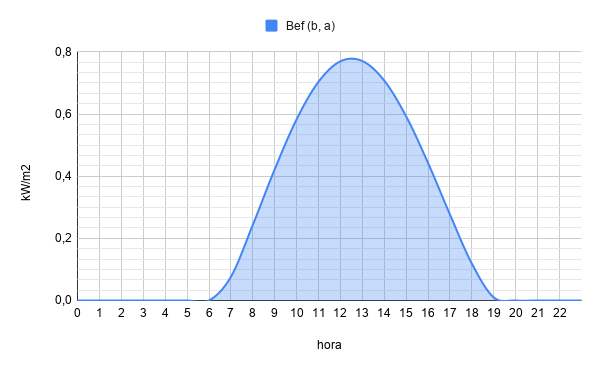
\includegraphics[scale=0.5]{bef}
\centering
\caption{Irradiancia directa efectiva en el plano inclinado}
\label{fig:hourly_bef}
\end{figure}

\begin{figure}[H]
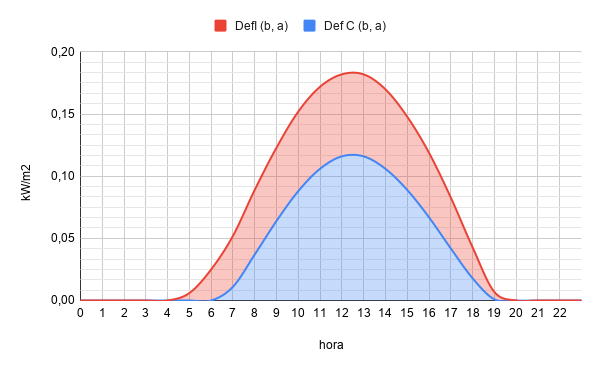
\includegraphics[scale=0.5]{defc_defi}
\centering
\caption{Componentes de la irradiancia difusa efectiva en el plano inclinado}
\label{fig:hourly_defc_defi}
\end{figure}

\begin{figure}[H]
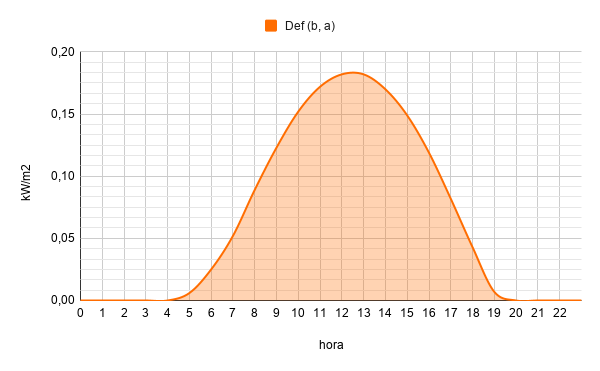
\includegraphics[scale=0.5]{def}
\centering
\caption{Irradiancia difusa efectiva en el plano inclinado}
\label{fig:hourly_def}
\end{figure}

\begin{figure}[H]
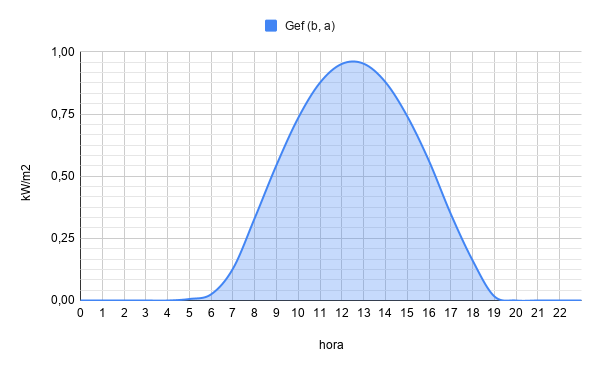
\includegraphics[scale=0.5]{gef}
\centering
\caption{Irradiancia global efectiva en el plano inclinado}
\label{fig:hourly_gef}
\end{figure}

Como se puede apreciar, los valores eficaces son ligeramente inferiores al aplicar las pérdidas por el nivel de suciedad medio y el ángulo de incidencia.

\subsection{Configuración del módulo solar y su comportamiento}

La primera parte del proceso de cálculo está completada, teniendo ya los valores eficaces de irradiancia horaria para cada uno de los 12 días promedio.

La segunda parte consiste en aplicar dicha radiación a un módulo para estimar la potencia máxima que será capaz de entregar, así como la energía que producirá al cabo de un año.

Para ello, tal y como se describe en el desarrollo teórico, debemos calcular la potencia en el punto de máxima potencia con las condiciones de temperatura y radiación del emplazamiento. Como ya tenemos los datos de radiación, a continuación calcularemos el perfil horario de temperatura como se describe en la sección de la página \pageref{section:term_behaviour}.

El resultado de ese proceso, para las coordenadas indicadas por el usuario se muestran en las tablas \ref{tab:temp_min_max} y \ref{tab:temp_profiles}.

\begin{table}[H]
\centering
\begin{tabular}{|c|r|r|r|r|r|r|r|r|r|r|r|r|}
\hline
$\degree C$ &
  \multicolumn{1}{c|}{Ene} &
  \multicolumn{1}{c|}{Feb} &
  \multicolumn{1}{c|}{Mar} &
  \multicolumn{1}{c|}{Abr} &
  \multicolumn{1}{c|}{May} &
  \multicolumn{1}{c|}{Jun} &
  \multicolumn{1}{c|}{Jul} &
  \multicolumn{1}{c|}{Ago} &
  \multicolumn{1}{c|}{Sept} &
  \multicolumn{1}{c|}{Oct} &
  \multicolumn{1}{c|}{Nov} &
  \multicolumn{1}{c|}{Dic} \\ \hline
$T_{min}$ & 0,7 & 2,6 & 5,8 & 8,9 & 11,8 & 17,5 & 22,4 & 18,6 & 14,1 & 10,8 & 6,8 & 4,9 \\ \hline
$T_{max}$ & 11,4 & 10,6 & 17,1 & 20,3 & 27 & 31,1 & 36,4 & 32,3 & 26,4 & 20,3 & 17,5 & 14,2 \\ \hline
\end{tabular}
\caption{Temperaturas máximas y mínimas en $\degree$C para cada uno de los 12 meses \label{tab:temp_min_max}}
\end{table}

\begin{figure}[H]
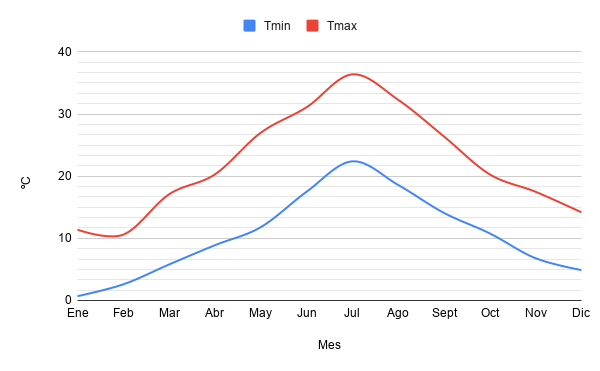
\includegraphics[scale=0.7]{tmax_tmin}
\centering
\caption{Temperaturas máximas y mínimas en $\degree$C para cada uno de los 12 meses}
\label{fig:temp_min_max}
\end{figure}

\begin{table}[H]
\centering
\begin{tabular}{|c|r|r|r|r|r|r|r|r|r|r|r|r|}
\hline
hora &
  \multicolumn{1}{c|}{Ene} &
  \multicolumn{1}{c|}{Feb} &
  \multicolumn{1}{c|}{Mar} &
  \multicolumn{1}{c|}{Abr} &
  \multicolumn{1}{c|}{May} &
  \multicolumn{1}{c|}{Jun} &
  \multicolumn{1}{c|}{Jul} &
  \multicolumn{1}{c|}{Ago} &
  \multicolumn{1}{c|}{Sept} &
  \multicolumn{1}{c|}{Oct} &
  \multicolumn{1}{c|}{Nov} &
  \multicolumn{1}{c|}{Dic} \\ \hline
0  & 1,05  & 3,14  & 7,19  & 11,04 & 15,46 & 21,13 & 25,96 & 21,43 & 15,86 & 11,57 & 7,21  & 5,11  \\ \hline
1  & 1,16  & 3,25  & 7,36  & 11,23 & 15,73 & 21,37 & 26,21 & 21,66 & 16,06 & 11,70 & 7,32  & 5,19  \\ \hline
2  & 1,56  & 3,60  & 7,93  & 11,84 & 16,54 & 22,09 & 26,95 & 22,39 & 16,69 & 12,14 & 7,73  & 5,51  \\ \hline
3  & 2,41  & 4,29  & 8,96  & 12,88 & 17,91 & 23,30 & 28,20 & 23,64 & 17,81 & 12,97 & 8,59  & 6,21  \\ \hline
4  & 3,83  & 5,37  & 10,46 & 14,34 & 19,76 & 24,91 & 29,89 & 25,37 & 19,43 & 14,26 & 10,03 & 7,44  \\ \hline
5  & 5,77  & 6,77  & 12,31 & 16,05 & 21,89 & 26,75 & 31,81 & 27,37 & 21,39 & 15,88 & 11,95 & 9,14  \\ \hline
6  & 7,88  & 8,23  & 14,18 & 17,74 & 23,94 & 28,50 & 33,65 & 29,34 & 23,36 & 17,58 & 14,04 & 11,02 \\ \hline
7  & 9,70  & 9,46  & 15,71 & 19,09 & 25,56 & 29,88 & 35,11 & 30,91 & 24,96 & 19,01 & 15,83 & 12,66 \\ \hline
8  & 10,88 & 10,25 & 16,68 & 19,93 & 26,56 & 30,73 & 36,01 & 31,88 & 25,96 & 19,90 & 16,99 & 13,73 \\ \hline
9  & 11,36 & 10,57 & 17,06 & 20,27 & 26,96 & 31,07 & 36,37 & 32,26 & 26,36 & 20,27 & 17,46 & 14,16 \\ \hline
10 & 11,39 & 10,59 & 17,08 & 20,28 & 26,98 & 31,08 & 36,38 & 32,28 & 26,38 & 20,29 & 17,49 & 14,19 \\ \hline
11 & 11,35 & 10,56 & 17,04 & 20,23 & 26,90 & 31,01 & 36,31 & 32,22 & 26,33 & 20,25 & 17,45 & 14,15 \\ \hline
12 & 11,33 & 10,54 & 17,01 & 20,20 & 26,86 & 30,97 & 36,27 & 32,18 & 26,30 & 20,23 & 17,43 & 14,14 \\ \hline
13 & 11,35 & 10,56 & 17,04 & 20,23 & 26,90 & 31,01 & 36,31 & 32,22 & 26,33 & 20,25 & 17,45 & 14,15 \\ \hline
14 & 11,39 & 10,59 & 17,08 & 20,28 & 26,98 & 31,08 & 36,38 & 32,28 & 26,38 & 20,29 & 17,49 & 14,19 \\ \hline
15 & 11,36 & 10,57 & 17,06 & 20,27 & 26,96 & 31,07 & 36,37 & 32,26 & 26,36 & 20,27 & 17,46 & 14,16 \\ \hline
16 & 10,88 & 10,25 & 16,68 & 19,93 & 26,56 & 30,73 & 36,01 & 31,88 & 25,96 & 19,90 & 16,99 & 13,73 \\ \hline
17 & 9,70  & 9,46  & 15,71 & 19,09 & 25,56 & 29,88 & 35,11 & 30,91 & 24,96 & 19,01 & 15,83 & 12,66 \\ \hline
18 & 7,88  & 8,23  & 14,18 & 17,74 & 23,94 & 28,50 & 33,65 & 29,34 & 23,36 & 17,58 & 14,04 & 11,02 \\ \hline
19 & 5,77  & 6,77  & 12,31 & 16,05 & 21,89 & 26,75 & 31,81 & 27,37 & 21,39 & 15,88 & 11,95 & 9,14  \\ \hline
20 & 3,83  & 5,37  & 10,46 & 14,34 & 19,76 & 24,91 & 29,89 & 25,37 & 19,43 & 14,26 & 10,03 & 7,44  \\ \hline
21 & 2,41  & 4,29  & 8,96  & 12,88 & 17,91 & 23,30 & 28,20 & 23,64 & 17,81 & 12,97 & 8,59  & 6,21  \\ \hline
22 & 1,56  & 3,60  & 7,93  & 11,84 & 16,54 & 22,09 & 26,95 & 22,39 & 16,69 & 12,14 & 7,73  & 5,51  \\ \hline
23 & 1,16  & 3,25  & 7,36  & 11,23 & 15,73 & 21,37 & 26,21 & 21,66 & 16,06 & 11,70 & 7,32  & 5,19  \\ \hline
\end{tabular}
\caption{Perfil de temperaturas en $\degree$C en las coordenadas del emplazamiento según el método descrito en \cite{temp_paper} \label{tab:temp_profiles}}
\end{table}

\begin{figure}[H]
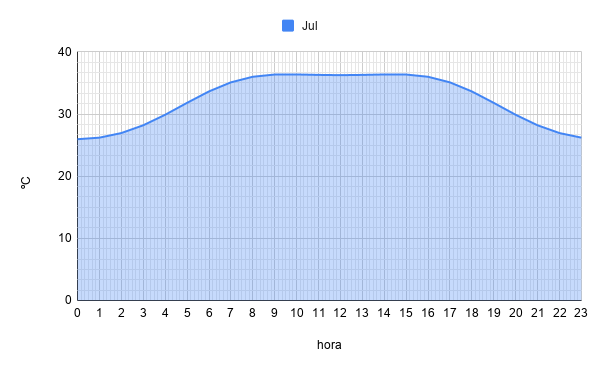
\includegraphics[scale=0.7]{july_temp}
\centering
\caption{Perfil horario de temperaturas para el día promedio del mes de Julio}
\label{fig:temp_min_max}
\end{figure}

La temperatura ambiente se necesita para calcular la temperatura de la célula según la ecuación \ref{eqn:T_c}, que a su vez se utiliza para calcular la tensión de circuito abierto, como se puede ver en la ecuación \ref{eqn:V_oc_cs}.

A continuación, en la tabla \ref{tab:mpp_values} se muestran los resultados del proceso de calculo descrito a partir de la página \pageref{section:var_form_factor} para hallar la tensión de circuito abierto $V_{oc}$, la intensidad de cortocircuito $I_{sc}$, asi como la tensión, intensidad y potencia en el punto de máxima potencia, todo ello en las condiciones de temperatura y radiación del emplazamiento indicado por el usuario
\newpage

\begin{table}[H]
\centering
\begin{tabular}{|c|r|r|r|r|r|r|}
\hline
 hora &
  \multicolumn{1}{c|}{$V_{oc} (V)$} &
  \multicolumn{1}{c|}{$I_{sc} (A)$} &
  \multicolumn{1}{c|}{$V_{mpp} (V)$} &
  \multicolumn{1}{c|}{$I_{mpp} (A)$} &
  \multicolumn{1}{c|}{$P_{mpp}(W)$} &
  \multicolumn{1}{c|}{$P_{ac}(W)$}\\ \hline
0  & 46,601 & 0 & 44,793 & 0 & 0 & 0			  \\ \hline
1  & 46,595 & 0 & 44,786 & 0 & 0 & 0  			  \\ \hline
2  & 46,578 & 0 & 44,767 & 0 & 0 & 0             \\ \hline
3  & 46,550 & 0 & 44,734 & 0 & 0 & 0             \\ \hline
4  & 46,512 & 0 & 44,689 & 0 & 0 & 0             \\ \hline
5  & 46,463 & 0,052 & 44,586 & 0,051 & 2,287 & 0  \\ \hline
6  & 46,405 & 0,222 & 44,365 & 0,220 & 9,782 & 6,531  \\ \hline
7  & 46,286 & 1,126 & 43,417 & 1,116 & 48,451 & 43,754  \\ \hline
8  & 46,093 & 2,935 & 41,575 & 2,906 & 120,800 & 112,216 \\ \hline
9 & 45,902 & 4,860 & 39,635 & 4,806 & 190,477 & 176,765\\ \hline
10 & 45,739 & 6,567 & 37,925 & 6,487 & 246,037 & 227,312 \\ \hline
11 & 45,619 & 7,842 & 36,652 & 7,742 & 283,740 & 261,161 \\ \hline
12 & 45,554 & 8,525 & 35,970 & 8,413 & 302,612 & 277,969\\ \hline
13 & 45,553 & 8,531 & 35,963 & 8,419 & 302,759 & 278,100\\ \hline
14 & 45,615 & 7,868 & 36,624 & 7,767 & 284,452 & 261,796 \\ \hline
15 & 45,732 & 6,636 & 37,856 & 6,556 & 248,184 & 229,249\\ \hline
16 & 45,895 & 5,009 & 39,495 & 4,953 & 195,606 & 181,469 \\ \hline
17 & 46,089 & 3,192 & 41,341 & 3,159 & 130,596 & 121,378 \\ \hline
18 & 46,290 & 1,429 & 43,151 & 1,416 & 61,081 & 55,820  \\ \hline
19 & 46,454 & 0,153 & 44,484 & 0,151 & 6,732 & 3,576  \\ \hline
20 & 46,512 & 0 & 44,689 & 0 & 0 & 0   \\ \hline
21 & 46,550 & 0 & 44,734 & 0 & 0 & 0   \\ \hline
22 & 46,578 & 0 & 44,767 & 0 & 0 & 0   \\ \hline
23 & 46,595 & 0 & 44,786 & 0 & 0 & 0   \\ \hline
\end{tabular}
\caption{Valores horarios de $V_{oc}$, $I_{sc}$, $I_{mpp}$, $V_{mpp}$ y $P_{mpp}$ para el día promedio del mes de julio } \label{tab:mpp_values}}
\end{table}

\begin{figure}[H]
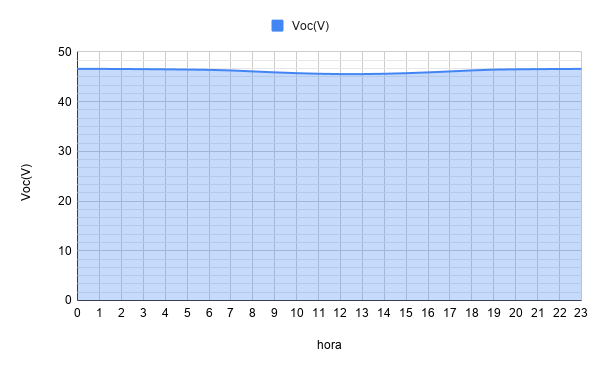
\includegraphics[scale=0.7]{Voc}
\centering
\caption{Valores horarios de tensión de circuito abierto para el día promedio del mes de Julio}
\label{fig:Voc}
\end{figure}

\begin{figure}[H]
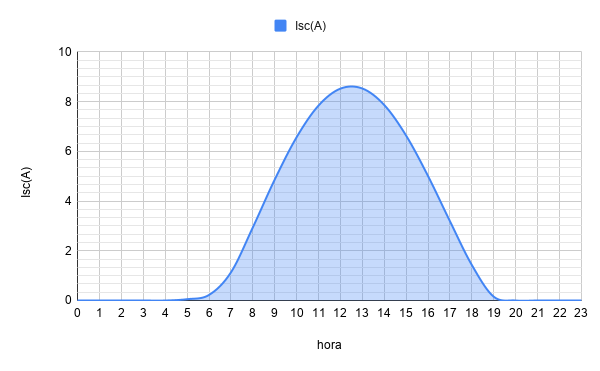
\includegraphics[scale=0.7]{Isc}
\centering
\caption{Valores horarios de corriente de cortocircuito para el día promedio del mes de Julio}
\label{fig:isc}
\end{figure}

\begin{figure}[H]
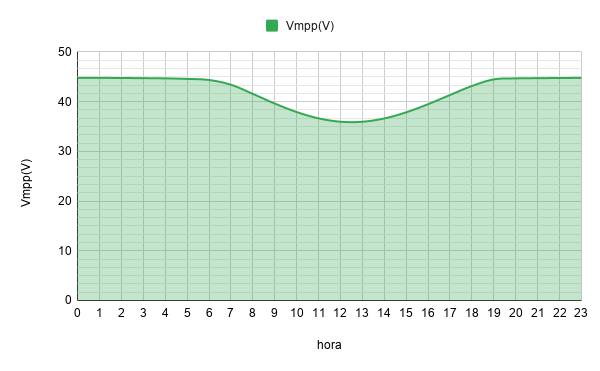
\includegraphics[scale=0.7]{Vmpp}
\centering
\caption{Valores horarios de tensión en el punto de máxima potencia para el día promedio del mes de Julio}
\label{fig:vmpp}
\end{figure}

\begin{figure}[H]
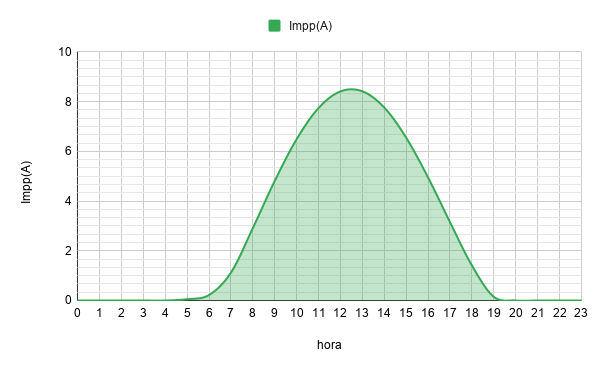
\includegraphics[scale=0.7]{Impp}
\centering
\caption{Valores horarios de corriente en el punto de máxima potencia para el día promedio del mes de Julio}
\label{fig:impp}
\end{figure}

\begin{figure}[H]
\includegraphics[scale=0.7]{Pmpp_pac}
\centering
\caption{Valores horarios de potencia en el punto de máxima potencia y a la salida del inversor para el día promedio del mes de Julio}
\label{fig:pmpp}
\end{figure}

\section{Cálculo final de las potencias y energías}

Habiendo hecho un breve repaso por el proceso de cálculo en un emplazamiento concreto, lo último y más importante que debemos estudiar son los resultados finales que se han obtenido, es decir, las potencias máximas mensuales, la productividad y sobretodo la energía, tanto mensual como anual, que es capaz de producir el generador configurado por el usuario.

Hasta el momento, con el fin de simplificar los cálculos, éstos se llevaron a cabo con un solo módulo. A continuación vamos a trasladar todos estos valores a la superficie que el usuario va a destinar para la instalación del generador.

Para ello, debemos obtener una relación entre el área disponible que el usuario ha introducido y el área total del generador configurado (12 módulo en serie y 11 en paralelo). Para ello, utilizamos el número total de módulos del generador base multiplicado por el área del un módulo, que se indica como uno de los valores disponibles en la tabla \ref{tab:module_conf}. 

En esta caso, la relación resultante es: 
\begin{equation}
\begin{align*}
Area_{generador} &= 12 \cdot 11 \cdot 1,941 m^2 = 256,257 m^2 \\
Area_{superficie} &= 40 m^2 \\
R &= \frac{Area_{superficie}}{Area_{generador}} = 0,156
\end{align*}
\end{equation}

Por otro lado, podemos obtener el numero de módulos totales que se pueden instalar en el área indicada por el usuario simplemente dividiendo el área indicada por el área de un módulo y redondeando hacia bajo al primero numero entero. De tal manera que:

\begin{equation}
\begin{align*}
Area_{modulo} &=  1,941 m^2 \\
Area_{superficie} &= 40 m^2 \\
N_{modulos} &= \frac{40}{1,941} = 20,60 \simeq 20
\end{align*}
\end{equation}

Por tanto, al conocer el numero de módulos, también podemos conocer la potencia nominal instalada, así como el resto de valores como la energía mensual, la potencia máxima que es capaz de entregar el generador o la productividad.

A continuación se muestran unos gráficos extraídos directamente de la página de resultados:

\begin{figure}[htbp]
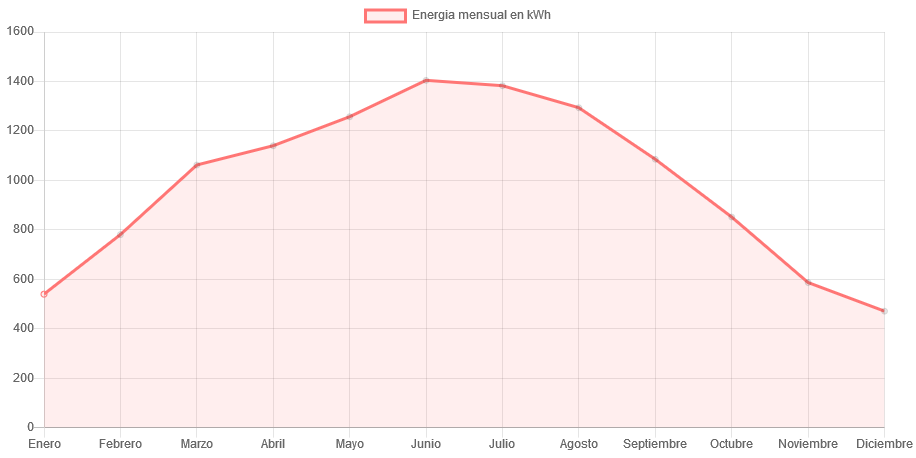
\includegraphics[scale=0.4]{monthly_energy}
\centering
\caption{Energía mensual producida}
\label{fig:fig_energy}
\end{figure}

\begin{figure}[htbp]
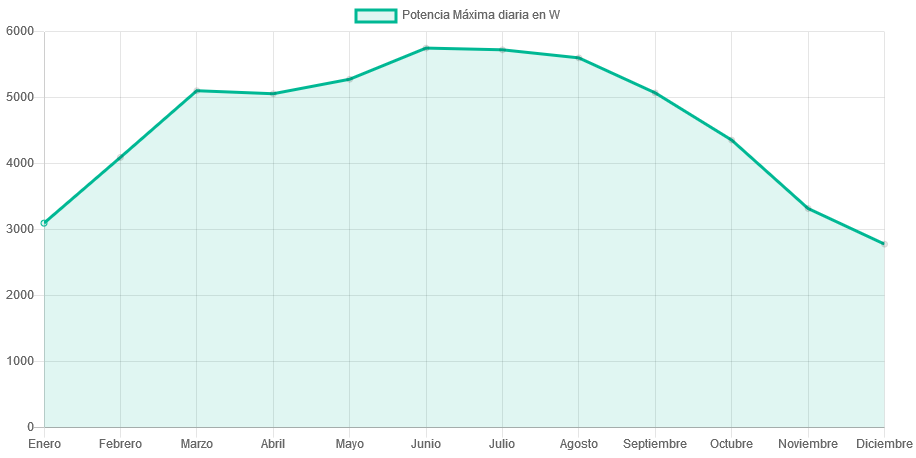
\includegraphics[scale=0.4]{monthly_power}
\centering
\caption{Potencia máxima mensual entregada}
\label{fig:fig_power}
\end{figure}

\begin{figure}[htbp]
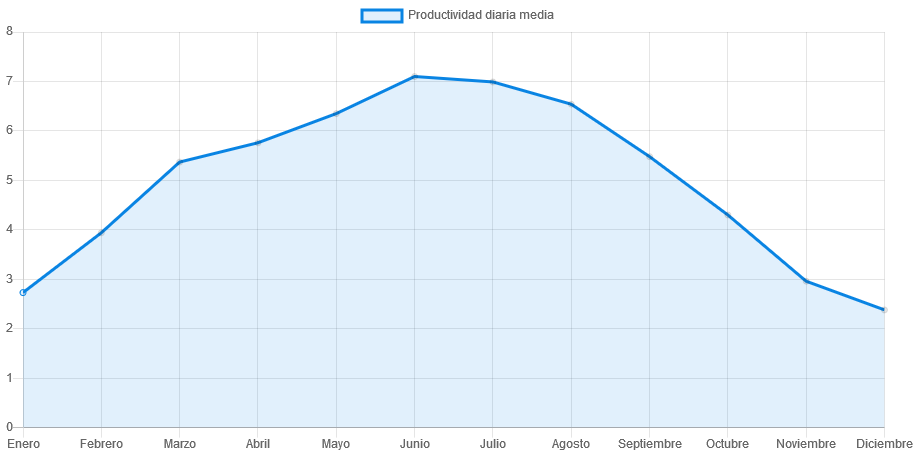
\includegraphics[scale=0.4]{monthly_productivity}
\centering
\caption{Productividad media mensual}
\label{fig:fig_prod}
\end{figure}
